\section{Transformationsrekonstruktion bei MeSH-Graphen}
\label{sec:vergleichBaume}
In diesem Kapitel wird die Vorgehensweise zur automatischen Rekonstruktion von Transformationen besprochen, welche zwei MeSH-Graphen ineinander überführen. Zuerst spezifizieren und diskutieren wir die Problemstellung. Danach stellen wir unseren Algorithmus vor und bewerten ihn.

% 1. Problembeschreibung -> Spezifikation
% 2. Erklärung der grundsätzlichen Probleme dieser Aufgabe
% 3. daraus resultierende Motivation der Spezifikation
% 4. Angabe eines Algorithmus' 
% ... -> entsprechende Entscheidungsbäume
% 5. Analyse des Algorithmus'
% ... -> warum ist es so richtig?

\subsection{Spezifikation}
\label{sec:formale_Beschreibung}
\begin{description}
 \item [Gegeben:] Zwei MeSH-Graphen $S$ und $T$, entsprechend \autoref{sec:repräsentation_des_mesh_als_baum}.
 \item [Gesucht:] Folge von Transformationen $O$, entsprechend \autoref{sec:mesh_operationen}, so dass $O(S) = T$, mit minimalem $|O|$.
\end{description}

%Gegeben seien zwei MeSH-Graphen $S$ und $T$. Gesucht ist eine Folge von Transformationen $O$ entsprechend \autoref{sec:mesh_operationen}, so dass folgende Bedingungen %
%erfüllt sind:
%\begin{itemize}
% \item $O(S) = T$
% \item $|O|$ ist minimal
 %\item jede Tree-Vertex und jeder Desriptor aus $S$ nur Operand einer Transformation $o$ aus  \todo{was ist ein Operand...?}
% \item mehr \todo{mehr Spezifikation!}
%\end{itemize}

\subsection{Motivation der Spezifikation}
Bei der Rekonstruktion der Überführung eines MeSH-Trees sind wir mit mehreren Problemen konfrontiert:
%[TODO: bespreche Problem der uneindeutigkeit. warum minimal? was ist minimal? wieso wird es minimal?]

\begin{description}
 \item[Nichteindeutigkeit der Lösung:] Ohne die Forderung der Minimalität von $|O|$ existieren unendlich viele Lösungen (z.\,B. durch wiederholtes Hinzufügen und Löschen des gleichen Descriptors). Die Forderung einer Transformationsfolge (anstelle einer Menge von Transformationen) ist notwendig, da Transformationen im Allgemeinen nicht kommutativ sind. Durch die Forderung der Minimalität sind allerdings bestimmte Gruppen von Transformationen kommutativ (siehe \autoref{sec:trans_prop}). Damit ist im Allgemeinen die Lösung nicht eindeutig.
%Auch mit der Forderung  Im Allgemeinen gibt es eine Vielzahl an möglichen Lösungen. Zum einen gibt es keinen harten Grund, dass es nur genau einen Weg gibt $S$ in $T$ mit einer festen Anzahl an Transformationen zu überführen. Zum anderen Suchen wir eine Folge von Transformationen. Vertauscht man die Reihenfolge zweiter Transformationen der Folge erhält man eine andere Lösung - selbst dann, wenn 

 \item[Nichteindeutigkeit des Problems:] Während wir sicherstellen können, dass immer eine Transformationsfolge gefunden wird die $S$ in $T$ überführt, sind wir nicht in der Lage die Qualität der Lösung objektiv einzuschätzen, da keine Musterlösungen vorliegen bzw. das tatsächliche Problem selbst nicht exakt formal darstellbar ist. Mit anderen Worten: es gibt keine streng rationale Vorgehensweise der Wissenschaftler am NLM nach der sie den MeSH verändern, da der MeSH kontinuierlich den realen Anforderungen und Entwicklungen der Wissenschaft angepasst wird. Entsprechend kann auch kein Algorithmus diesen Vorgang nachvollziehen. Stattdessen versuchen wir eine formale Spezifikation anzugeben, die dem realen Problem möglichst gerecht wird. 

 \item[Vermischung von Theorie und Anwendung:] Aus den vorangegangenen Punkten ergibt sich, dass wir auf Heuristiken angewiesen sind, welche sich nur durch domänenspezifische Plausibilitätsargumente motivieren lassen.
\end{description}

%Die obige Problem beschreibt versucht dennoch das Problem möglichst formal zu fassen.
%Trotz dieser Schwierigkeiten geben wir nachfolgend eine möglichst formale Beschreibung eines Algorithmus' an:

%Wir fordern die Minimalität von $|O|$, denn daraus folgt: (i) die Kommutativität von Transformationen entsprechend \autoref{sec:trans_prop}. Kommutativität erleichtert das  und (ii) das Vermeiden überflüssiger Transformationen. \todo{genauer}
%TODO: folgt aus der minimalität von |O| die Kommutativität von O ? das wäre echt cool!
% was soll das eigentlich.
% PRIMÄRE FRAGE SOLLTE LAUTEN: wie bekomme ich das hier schnell fertig!

%Die zweite Einschränkung verhindert, dass Transformationen gestückelt durch
%Wir suchen hingegen solche Transformationen $O$, die nur solche Änderungen durchführen, die auch notwendig sind. \par  

%Wir suchen also eine Transformationsfolge $O$ die $S$ in $T$ überführt und minimal lang ist. Diese Einschränkung ist wichtig, da es trivial ist ein beliebiges $O$ zu finden: man wählt $O$ so, dass es alle Descriptors und Tree Vertices aus $S$ entfernt und danach alle Descriptors und Tree Vertices aus $T$ einfügt. 

\subsection{Algorithmus}
%\subsubsection{Übersicht}
Zusammenfassend ist die Vorgehensweise des Algorithmus' die Folgende: Wir gehen von $T$ aus und durchlaufen all dessen Descriptors bzw. Tree Vertices, um nacheinander für jeden Descriptor bzw. jede Tree Vertex die Transformation zu bestimmen, durch die dieser Descriptor bzw. diese Tree Vertex in $T$ vorhanden ist. Zur Bestimmung einer konkreten Transformation verwenden wir Entscheidungsbäume. Dabei vergleichen wir ob bzw.\ wie $S$ und $T$ lokal übereinstimmen und leiten daraus die durchgeführte Transformation ab. \par

%Das uns für diese Aufgabe zur Verfügung stehende Wissen ist ausschließlich: 
%\begin{itemize}
%  \item die beiden MeSH-Graphen $S$ und $T$
%  \item Menge der zulässigen Transformationen auf MeSH-Graphen.
%  \item Domänen-Wissen zum MeSH mit dem heuristische Entscheidungen begründet werden. Darauf wird gegebenenfalls konkret hingewiesen.
%   %heuristisches Wissen Wissen darüber, welche Transformationen auf welche Art und Weise im Kontext des MeSH Sinn ergeben
%\end{itemize}

Wie in \ref{sec:mesh_operationen} \textit{\nameref{sec:mesh_operationen}} beschrieben, existieren verschiedene Transformationstypen. Wir bestimmten die konkreten Transformation in folgender Reihenfolge:
\begin{enumerate}
  \item Descriptor-Additionen, Descriptor-Relabellings, Descriptor-Umbenennungen
  \item Vertex-Neuverknüpfungen
  \item Vertex-Verschiebungen, Vertex-Umbenennungen, Vertex-Additionen
  \item Descriptor-Löschungen, Vertex-Löschungen
\end{enumerate} 

Die Reihenfolge ergibt sich aus dem Algorithmus, wie folgt:
\begin{itemize}
 \item Descriptors und Tree-Vertices werden als gelöscht erkannt, genau dann, wenn sie nicht als anderweitig verändert erkannt wurden. Folglich müssen Löschungen nach allen anderen Transformationen bestimmt werden.
 \item Die beiden Entscheidungsbäume für Vertex-Transformationen (für 2. und 3. oben) setzen voraus, dass alle Descriptor-Transformationen bekannt sind. Daher werden Descriptor-Transformationen vor Vertex-Transformationen bestimmt.
 \item Die Reihenfolge von 2. und 3. ist beliebig.
\end{itemize}

Innerhalb der obigen Schritte gehen wir iterativ vor, wie in nachfolgenden Abschnitten für die einzelnen Transformationstypen beschrieben wird. Der Pseudocode in \autoref{lst:tree_compare_pseudocode} veranschaulicht das Vorgehen.

\lstset{caption=Algorithmus zur Transformationsrekonstruktion}
\lstset{label=lst:tree_compare_pseudocode}
\begin{lstlisting}[float=htbp] 
Eingabe: MeSH-Graph S (Ausgangsgraph), MeSH-Graph T (Zielgraph)

// Initialisierung
leere O 
setze VT gleich der Menge aller Tree-Vertices in T
setze VS gleich der Menge aller Tree-Vertices in S
setze DS gleich der Menge aller Descriptors in S
setze DT gleich der Menge aller Descriptors in T

// Descriptor-Transformationen (außer Löschungen)
für alle (dT in DT):
  bestimme Transformation o die zum Auftreten von dT in T führt
  füge o an O an

// Vertex-Rebindings
für alle (vT in VT):
  wenn (vT ist Resultat eines Vertex-Rebindings)
    bestimme diese Transformation o
    füge o an O an

// Vertex-Transformationen (außer Löschungen)
traversiere MeSH-Tree of T mit Tiefensuche, sei vT das aktuelle Element:
  bestimme Transformation o die zum Auftreten von vT in T führt
  füge o an O an

// Descriptor-Löschungen
für alle (dS in DS):
  wenn (dS wurde aus S gelöscht um T zu erzeugen)
    füge diese Löschung an O an  

// Vertex-Löschungen
für alle (vS in VS):
  wenn (vS wurde aus S gelöscht um T zu erzeugen)
    füge diese Löschung an O an

Ausgabe: Transformationssequenz O
\end{lstlisting} 

% \minisec{Veränderungen und Hinzufügen}
% \begin{itemize}
%   \item[] $O:=\emptyset$  \% O ist Folge der bestimmten Transformationen
%   \item[] $U:=\emptyset$  \% U ist Menge der 'verbrauchten' Descriptors
%   \item[] $D_T = \text{Set of all Descriptors of }T$
%   \item[] $D_S = \text{Set of all Descriptors of }S$
%   \item[] forall $d_T \in D_T$:
%   \begin{itemize}
%     \item[] if $\left( \exists d_S \in D_S / used \text{ : } \exists op \in Op \text{ : } op(d_S) = d_T \wedge isValid(op) \right)$ :
%     \begin{itemize}
%       \item[] $O := O \cup \{op(d_S)\}$
%       \item[] $used := used + \{d_S\}$
%      \end{itemize}
%     \item[] else
%     \begin{itemize}
%       \item[] $O := O \cup \{descAdd(d_T)\}$
%      \end{itemize}
%   \end{itemize}
% \end{itemize}
% 
% \minisec{Löschungen}
% \begin{itemize}
%   \item[] forall $d_S \in DS / used$ :
%   \begin{itemize}
%     \item[] $O := O \cup \{descDel(d_S) \}$
%    \end{itemize}
% \end{itemize}

\subsection{Vorgehen für Transformationstypen}

\minisec{Bezeichnungen}
Es folgen Erläuterungen zu den Bezeichnungen in diesem Abschnitt. \par

\begin{tabular}{rl}
   \code{vT} & gerade betrachtete Tree Vertex aus \code{T} \\
   \code{vS} & Entsprechung \code{vT}\,s in \code{S}, also \code{vT}\,s Ursprung \\
   \code{dT} & Descriptor \code{vT}\,s in \code{T}, bzw. gerade betrachteter Descriptor \\
   \code{dS} & Descriptor \code{vS}\,s in \code{S} \\ \\
   \code{dad(v)} & Vater der Tree Vertex \code{v} \\
   \code{name(d)} & Name eines Descriptors \code{d} \\
   \code{ui(d)} & UI eines Descriptors \code{d} \\ \\
   \code{S(ui)} & Descriptor in \code{S} der UI \code{ui} besitzt\\
   \code{S(dname)} & Descriptor in \code{S} der Name \code{dname} besitzt\\
   \code{S(vname)} & Tree Vertex in \code{S} der Name \code{vname} besitzt\\ 
\end{tabular}

\subsubsection{Descriptor-Transformationen}
Um alle Transformationen der Descriptors (außer Löschungen) herauszufinden, traversieren wir die Menge der Descriptors in beliebiger Reihenfolge und nehmen dann eine Fallunterscheidung vor, wie in \autoref{fig:compare_descMods} dargestellt. \par

\begin{figure}[h]
\begin{center}
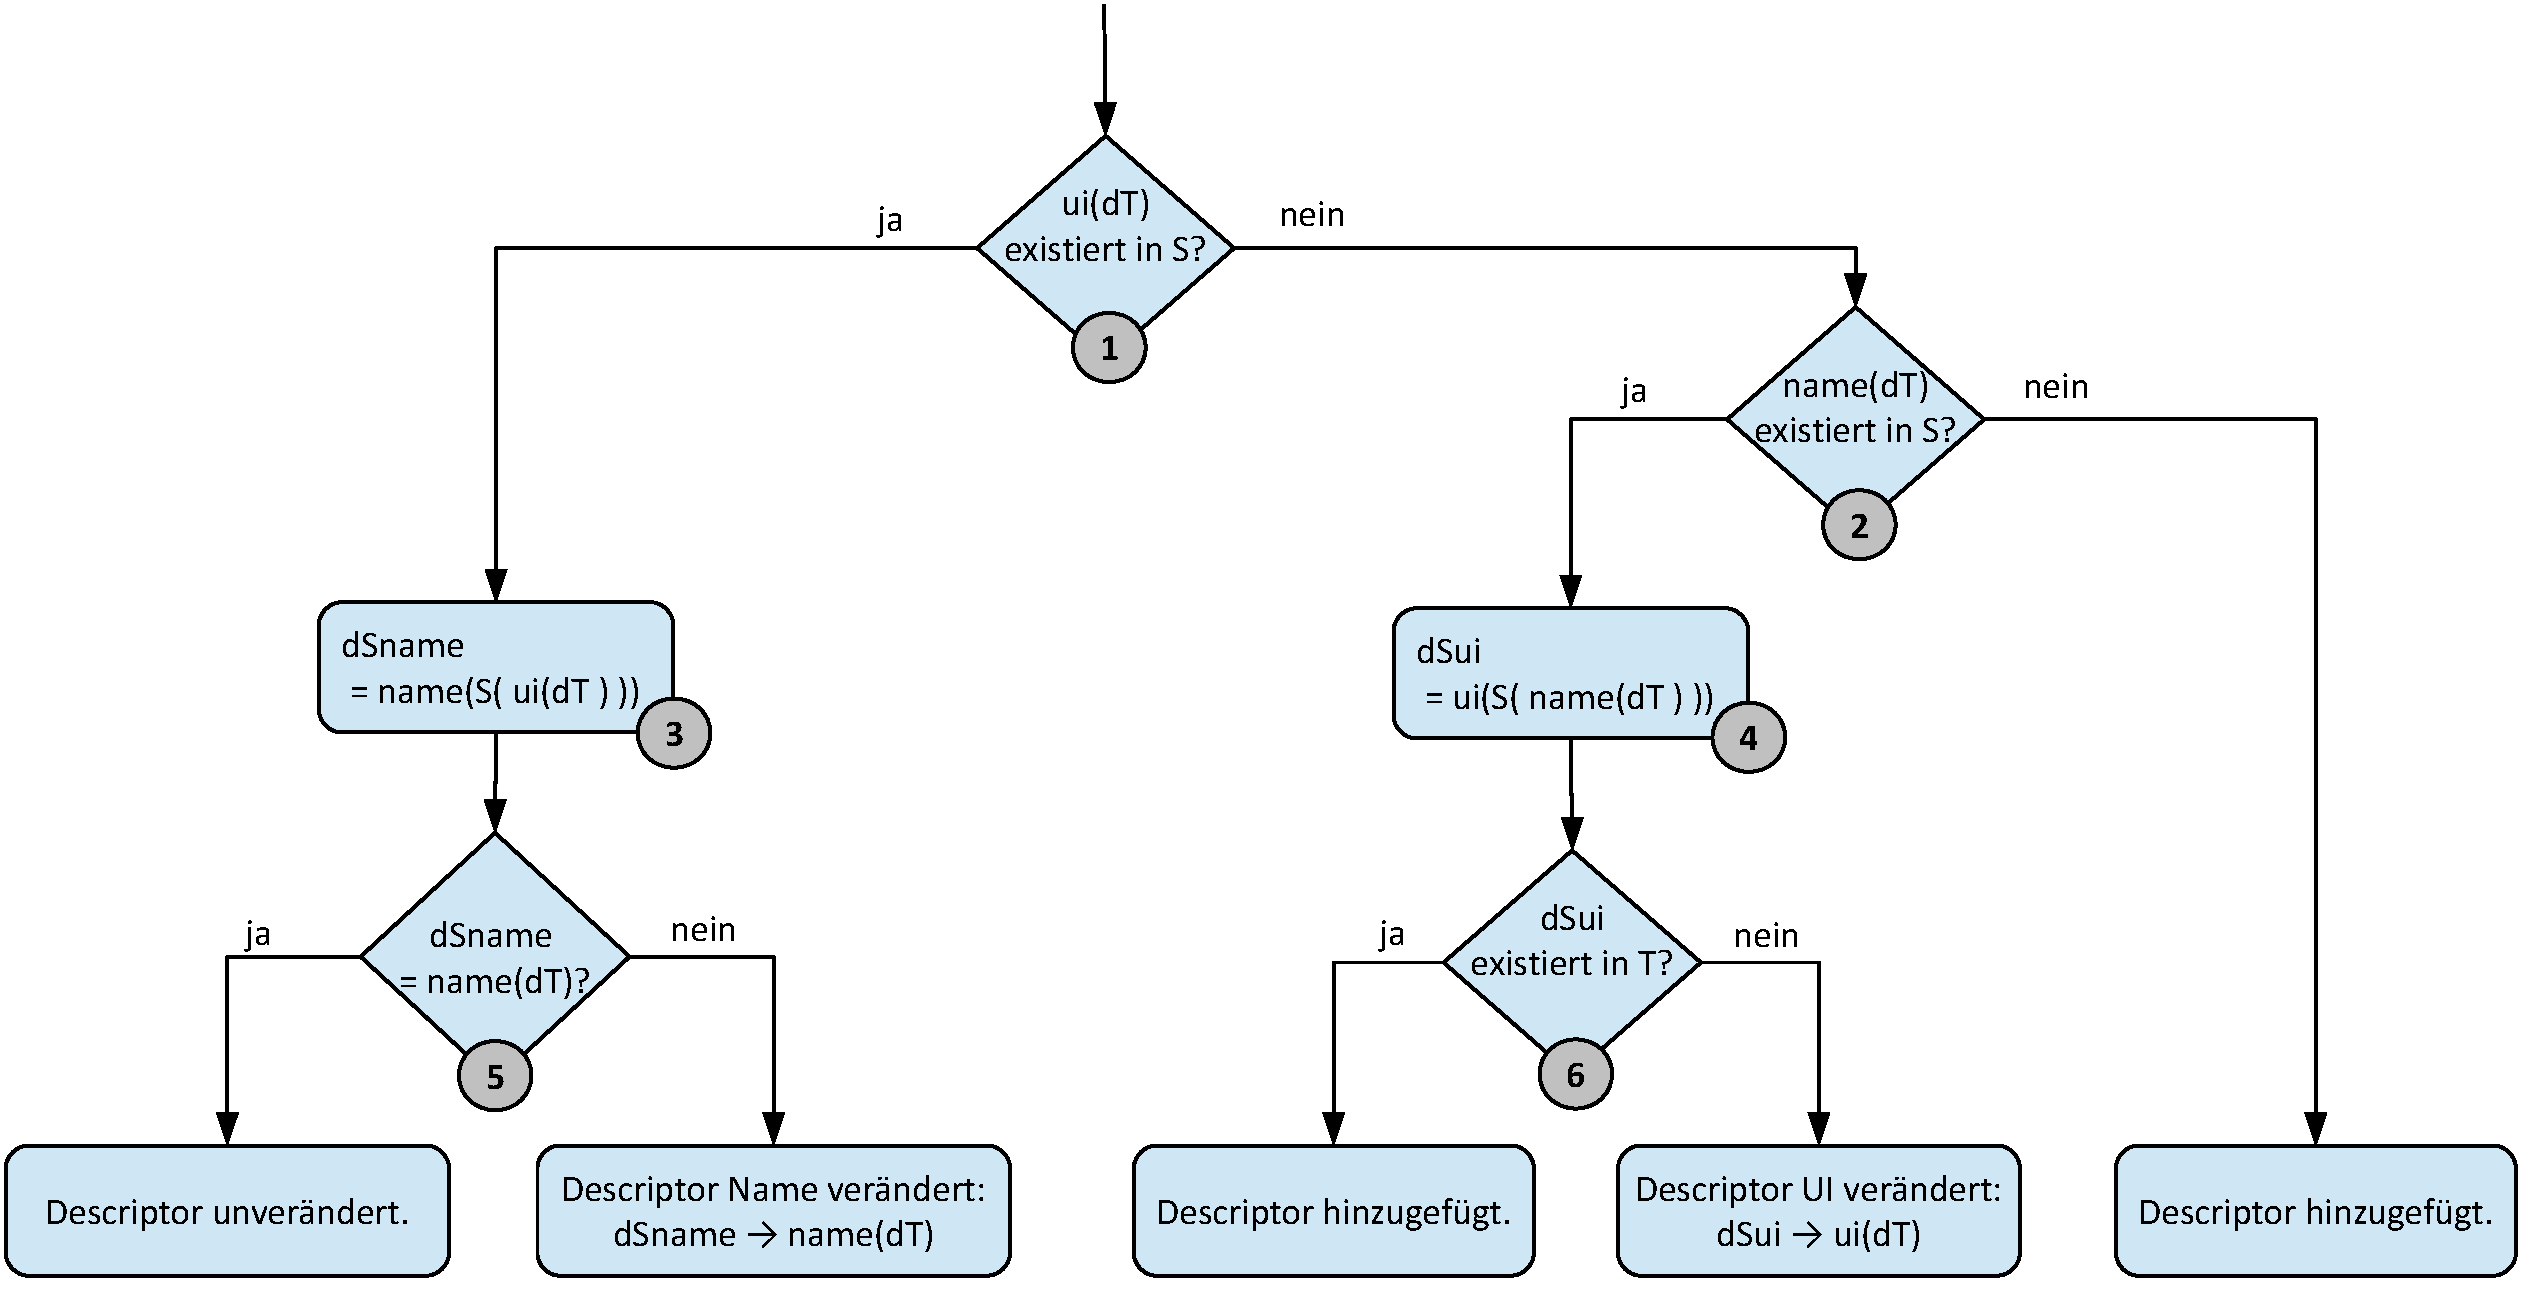
\includegraphics[width=1.05\textwidth]{figs/compare_descMods.pdf}
\end{center}
\caption{Bestimmen der Transformationen auf Descriptors}
\label{fig:compare_descMods}
\end{figure}

Es folgen Erklärungen zu den einzelnen Schritten in \autoref{fig:compare_descMods}.
\begin{enumerate}
  \item[(1)] überprüft, ob es in \code{S} einen Descriptor mit selber UI wie \code{dT} gibt.
  \item[(2)] überprüft, ob es in \code{S} einen Descriptor mit selbem Namen wie \code{dT} gibt. Wenn auch dies nicht der Fall ist, dann ist \code{dT} ein neuer Descriptor.
  \item[(3)] Für Leserlichkeit: setzt \code{dSname} gleich dem Namen des Descriptors in \code{S}, der die selbe UI wie \code{dT} hat.
  \item[(4)] Für Leserlichkeit: setzt \code{dSui} gleich der UI des Descriptors in \code{S}, der den selben Namen wie \code{dT} hat.
  \item[(5)] überprüft, ob neben der UI auch der Name \code{dT}\,s und \code{S(ui(dT))}\,s übereinstimmt. Wenn dem so ist, dann ist \code{dT} unverändert. Ansonsten hat sich der Name von \code{dSname} zu \code{name(dT)} geändert. Siehe dazu auch die Anmerkungen im nachfolgenden Abschnitt \textit{Aufteilen eines Descriptors}.
  \item[(6)] überprüft, ob es einen Descriptor \code{dS} mit UI \code{dSui} in \code{T} gibt. Ist dies der Fall, dann ist \code{dT} entstanden, indem der Name \code{dS}\,s geändert wurde. Ansonsten existiert also kein "`ähnlicher"' Descriptor in \code{S}, folglich ist \code{dS} hinzugefügt wurden. Siehe dazu auch die Anmerkungen im nachfolgenden Abschnitt \textit{Aufteilen eines Descriptors}.
\end{enumerate}

\minisec{Aufteilen eines Descriptors}
\label{sec:aufteilung_descriptor}

\begin{figure}[h]
\begin{center}
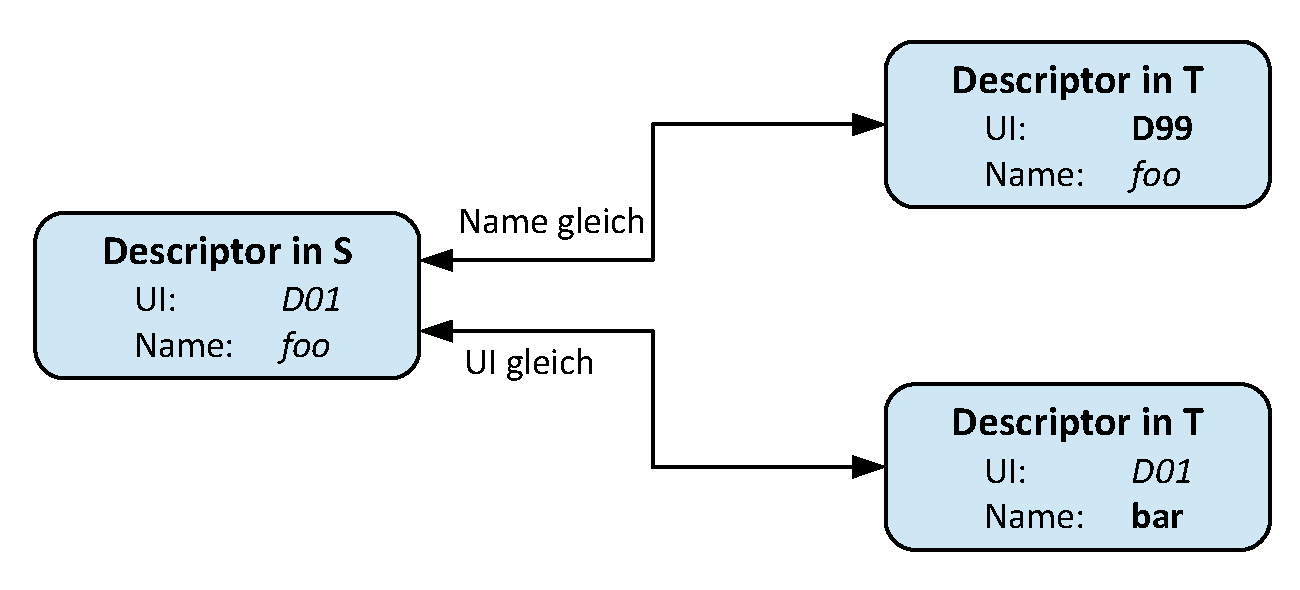
\includegraphics[width=0.7\textwidth]{figs/compare_descSplitting.pdf}
\end{center}
\caption{Descriptor-Aufteilung}
\label{fig:compare_descSplitting}
\end{figure}

Sei \code{(x,y)} für diesen Abschnitt die Bezeichnung für einen Descriptor mit UI \code{x} und Name \code{y}. Bei der Bestimmung der Descriptor-Transformationen zweier MeSH-Trees \code{S} und \code{T} kann es zu der in \autoref{fig:compare_descSplitting} gezeigten Situation kommen: Beide Descriptors aus \code{T}, \code{(D01,bar)} und \code{(D99,foo)}, sind potentiell aus \code{(D01,foo)} aus \code{S} entstanden. Wir müssen uns für der beiden Überführungsmöglichkeiten entscheiden:
%. Allerdings kann \code{(D01,foo)} nicht Operand verschiedener Transformationen sein, da es sonst zwei Transformationen geben würde, die auf \code{(D01,foo)} angewendet werden würden, was die Spezifikation aus \autoref{sec:formale_Beschreibung} verbietet. Man muss sich also für eine der beiden folgenden Überführungsmöglichkeiten entscheiden:

\begin{enumerate}
  \item Descriptor \code{(D99,foo)} ist neu. Descriptor \code{(D01,bar)} ist durch Änderung des Namens \code{(D01,foo)}\,s entstanden.
  \item Descriptor \code{(D01,bar)} ist neu. Descriptor \code{(D99,foo)} ist durch Änderung der UI \code{(D01,foo)}\,s entstanden.
\end{enumerate}

Wir entscheiden uns aus heuristischen Gründen für Variante 1: Ein Term aus \code{(D01,foo)} wurde in einen neuen Descriptor verschoben ($\rightarrow$ \code{(D99,foo)}). Dieser Term war gerade der Preferred Term, weshalb sich der Name geändert hat ($\rightarrow$ \code{(D01,bar)}). Im Gegensatz dazu sehen wir keinen Grund, warum man im MeSH die UI eines Descriptors ändern sollte.  

\subsubsection{Vertex-Neuverknüpfung}
Vertex-Neuverknüpfungen, also das Verändern, zu welchem Descriptor eine Tree Vertex gehört, sind ein Spezialfall des Vertex-Verschiebens. Dieser Sonderfall ist in \ref{sec:mesh_operationen} \textit{\nameref{sec:mesh_operationen}} dargestellt.

%Entsprechend lassen sie sich weiter in 2 Klassen einteilen: Zum einen "`Pure"' Vertex Rebindings bei denen die Tree Vertex ihren Namen behält, und zum anderen Rebindings, bei denen sich auch ihr Name ändert. Letztere werden in \ref{sec_weitere_vertex_mods} \textit{\nameref{sec_weitere_vertex_mods}} behandelt. Hier geht es ausschließlich um Pure Vertex Rebindings.\par

Wir iterieren über alle die Tree Vertices \code{vT} in \code{T}, deren Namen sich nicht geändert haben, und erkennen eine Vertex-Neuverknüpfung, falls (i) weder Name noch UI der beiden Descriptors \code{dT} und \code{dS} übereinstimmen und es außerdem (ii) kein Descriptor Relabelling bzw. Descriptor Renaming gibt, welches \code{name(dS)} in \code{name(dT)} bzw. \code{ui(dS)} in \code{ui(dT)} überführt.\par

Die erste Bedingung ist evident, da sich bei einer Vertex-Neuverknüpfung gerade der Descriptor ändert. Die zweite Bedingung erklärt sich dadurch, dass ein Umbenennen oder Relabeln eines Descriptors zwar den Descriptor verändert, nicht aber eine Vertex-Neuverknüpfung für dessen Tree Vertices darstellt. \par   

\subsubsection{Weitere Vertex-Transformationen}
\label{sec_weitere_vertex_mods}

Um alle restlichen Vertex-Transformationen zu bestimmen, traversieren wir \code{T} mittels Tiefensuche und bestimmen dann für den jeweils aktuell betrachteten Tree Vertex \code{vT} mittels des in \autoref{fig:compare_vertexMods} skizzierten Vorgehens dessen Entsprechung \code{vS} in \code{S}.\par

Es ist dabei wichtig, dass der Baum in einer solchen Reihenfolge durchlaufen wird, die garantiert, dass alle Vorfahren der aktuellen Tree Vertex bereits durchlaufen wurden. Denn an verschiedenen Stellen wird vorausgesetzt, dass der Ursprung von \code{dad(vT)} bekannt und endgültig bestimmt ist. Offensichtlich erfüllt Tiefensuche dieses Kriterium. \par  

\begin{figure}[h]
\begin{center}
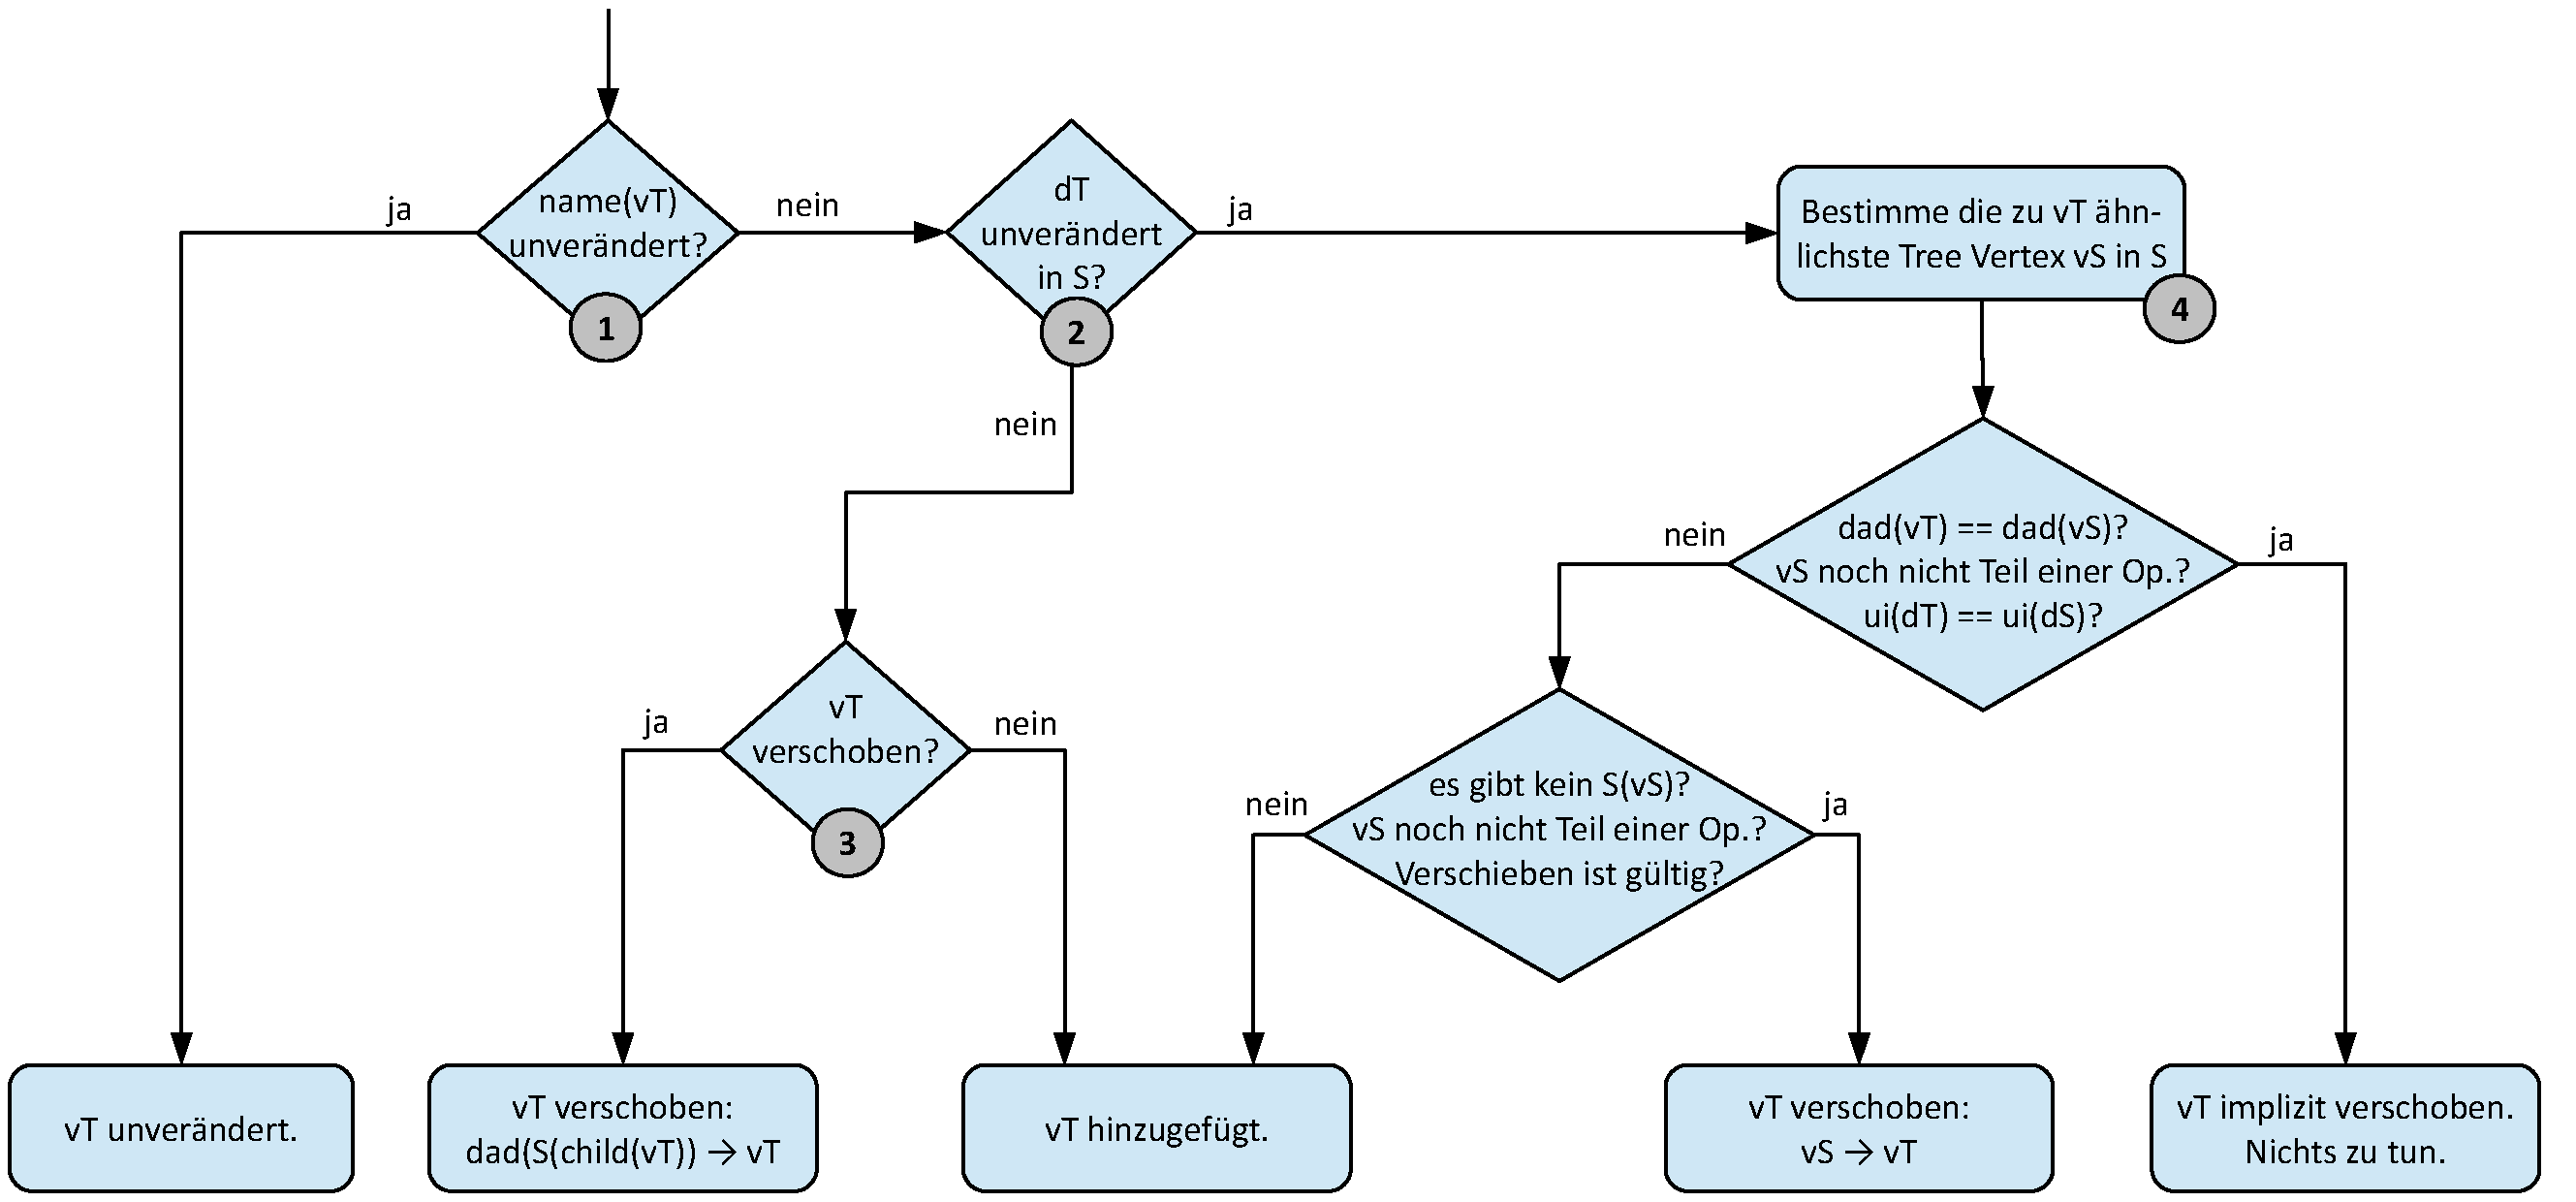
\includegraphics[width=1.05\textwidth]{figs/compare_vertexMods.pdf}
\end{center}
\caption{Bestimmen der Vertex-Transformationen}
\label{fig:compare_vertexMods}
\end{figure}

\minisec{Erläuterung von \autoref{fig:compare_vertexMods}}
% \begin{description}
% \item[\Large{\ding{172}}]% \normalsize{} Tree Vertex unverändert?]
% \end{description}

\begin{itemize}
\item[(1)] Hat sich der Name \code{vT}\,s verändert? Wenn nicht, dann hat sich auch seine Position im MeSH-Tree nicht verändert. Denn im MeSH beschreibt der Name einer Tree Vertex gerade seine Position. Wenn dies zutrifft, ist also nichts zu tun.

\item[(2)] Es wird überprüft, ob \code{dT}, also der Descriptor \code{vT}\,s, unverändert aus \code{S} übernommen wurde.

\item[(3)] %Descriptor verändert - Tree Vertex neu oder verschoben
Ist der Descriptor verändert worden, stehen wir vor einer schwierigen Aufgabe: Sowohl Descriptor als auch Tree Number \code{vT}\,s haben sich verändert. Dies sind aber die beiden wichtigsten Informationen, um herauszufinden, ob \code{vT} nun durch Verschieben oder Hinzufügen in \code{T} vorhanden ist. Es bleibt nur die strukturelle Information, d.\,h. wir analysieren die Kinder und Eltern \code{vT}\,s und versuchen daraus dessen Ursprung abzuleiten. Dabei gehen wir nach folgendem Prinzip vor:\par

\begin{itemize}
  \item[] Angenommen die Kinder \code{vT}\,s sind unverändert (d.\,h. nur implizit verschoben) und ein solches Kind sei \code{cT}.
  \item[] Wir bestimmen den Vater \code{cS}\,s, also den Vater der Entsprechung \code{cT}\,s in \code{S}, als die Tree Vertex des Descriptors \code{cS}\,s, die \code{vT} am ähnlichsten ist. Als Ähnlichkeitsmaß verwenden wir das in \ref{sec:tree_vertex_ähnlichkeit} \textit{\nameref{sec:tree_vertex_ähnlichkeit}} beschriebene. %\par
  \item[] Wenn nun \code{vT} auch in \code{S} der Vater \code{cS}\,s gewesen sein sollte, wenn \code{vT} also von dort zu seiner aktuellen Position verschoben wurde, dann müssten die \code{dad(cS)} für alle Kinder \code{cS} von \code{vT} übereinstimmen. Sollten die Eltern der Kinder in \code{S} jedoch nicht in ausreichendem Maß übereinstimmen, dann ist \code{vT} zu \code{T} hinzugefügt wurden.
\end{itemize}

%TODO Bild / weitere Erklärung \par
  
%Angenommen die Kinder \code{vT}\,s seien unverändert. Das heißt ihre Tree Number hat sich zwar verändert, aber nur weil einer ihrer Vorfahren verschobe wurde. Dann betrachten wir alle direkten Kinder \code{vT}\,s und bestimmen für jedes der \code{cT} dessen Ursprung \code{cS} (ebenfalls heuristisch).  
 

\item[(4)] %\minisec{Descriptor unverändert - Tree Vertex implizit verschoben, explizit verschoben oder hinzugefügt}  Zurück zur Fallunterscheidung zu \code{dT}.
Es existiert \code{dT} also unverändert in \code{S} als \code{dS}. Wir wollen nun den wahrscheinlichsten Ursprung \code{vT}\,s in \code{S}, also \code{vS}, bestimmen. Da \code{dT} unverändert ist, muss \code{vS} eine der Tree Vertices \code{dS}\,s sein. Wir wählen als \code{vS} jene Tree Vertex \code{dS}\,s die \code{vT} am ähnlichsten ist. Als Ähnlichkeitsmaß verwenden wir das in \ref{sec:tree_vertex_ähnlichkeit} \textit{\nameref{sec:tree_vertex_ähnlichkeit}} beschriebene. \par

Es sind nun drei Fälle zu unterschieden: 
\begin{enumerate}
  \item \code{vT} wurde implizit verschoben, das heißt sein Name (Tree Number) hat sich nur verändert, weil einer seiner Vorfahren verschoben wurde.
  \item \code{vT} wurde explizit verschoben.
  \item \code{vT} ist eine neue Tree Vertex eines existierenden Descriptor.
\end{enumerate} 

%\item[Descriptor unverändert - Tree Vertex implizit verschoben]
\textit{Fall 1} (\code{vT} wurde implizit verschoben) tritt ein, falls folgende Bedingungen erfüllt sind:
\begin{enumerate}
  \item \code{dad(vT) == dad(vS)}, d.\,h. \code{vT}\,s Vater ist gleich geblieben. 
  \item \code{ui(dT) == ui(dS)}, d.\,h. \code{vT}\,s Descriptor ist gleich geblieben. 
  \item \code{vS} ist nicht bereits Teil einer zuvor bestimmten Transformation.
\end{enumerate}

%\item[Descriptor unverändert - Tree Vertex explizit verschoben]
\textit{Fall 2} (\code{vT} wurde explizit verschoben) tritt ein, falls gilt:
\begin{enumerate}
  \item \code{vT} wurde nicht implizit verschoben.
  \item In \code{T} existiert keine Tree Vertex mit gleichem Namen wie \code{vS}, d.\,h. der zuvor bestimmte Ursprung \code{vT}\,s ist überhaupt ein möglicher Ursprung.
  \item \code{vS} ist nicht bereits Teil einer zuvor bestimmten Transformation.  
  \item \code{vS} ist kein Vorfahre der Entsprechung \code{dad(vT)}\,s in \code{S}, d.\,h. \code{vS} wird nicht nach einem Nachkommen seiner selbst verschoben. Denn das wäre keine gültige Transformation.   
\end{enumerate}

%\item[(5) Descriptor unverändert - Tree Vertex hinzugefügt]
\textit{Fall 3} (\code{vT} wurde hinzugefügt) tritt ein, falls Fall 1 und Fall 2 nicht eingetreten sind. 
%Falls \code{vT} auch nicht explizit verschoben wurde, so muss \code{vT} hinzugefügt worden sein.\par

\end{itemize}

\subsubsection{Tree-Vertex-Löschungen}
\label{sec:tree_vertex_del}
Um alle Tree-Vertex-Löschungen zu finden, gehen wir wie folgt vor: \par
Wenn ein Vertex \code{v} aus \code{S} nicht mehr unverändert in \code{T} vorkommt, und außerdem keine Transformation \code{v} in eine Tree Vertex in \code{T} überführt, dann muss \code{v} aus \code{S} gelöscht worden sein. \par
Aus diesem Vorgehen folgt unmittelbar, dass alle anderen Transformationen vor den Löschungen bestimmt werden müssen.

\subsubsection{Descriptor-Löschungen}
Das Prinzip ist analog zu dem in \autoref{sec:tree_vertex_del}: \par
Wenn ein Descriptor \code{d} aus \code{S} nicht mehr unverändert in \code{T} vorkommt, und außerdem keine Transformation \code{d} in einen Descriptor in \code{T} überführt, dann muss \code{d} aus \code{S} gelöscht worden sein.

%\subsection{Korrektheit und Optimale Lösung}
\subsection{Bewertung des Algorithmus}
Mit der hier dargestellten Vorgehensweise wird eine Transformationsfolge \code{O} gefunden, die \code{S} in \code{T} 
%entsprechend der Anforderungen aus \autoref{sec:formale_Beschreibung} 
überführt, denn:

\begin{itemize}
  \item jeder Descriptor \code{d} bzw. jede Tree Vertex \code{v} in \code{T} wird genau einmal durchlaufen.
  \item bei einem solchen Durchlaufen wird
  \begin{itemize}
    \item immer genau eine Transformation bestimmt, welche zum Auftreten von \code{d} bzw. \code{v} in \code{T} führt.
    \item keine zuvor gefundene Transformation gelöscht oder verändert.
    \item keine Transformation bestimmt, die in Widerspruch mit einer zuvor bestimmten Transformation stehen würde, d.\,h. \code{O(S)} ist zu jedem Zeitpunkt des Algorithmus' definiert.
  \end{itemize}
  \item jeder Descriptor \code{d} bzw. jede Tree Vertex \code{v} in \code{S}, die nicht durch eine zuvor ermittelte Transformation nach \code{T} übernommen wird, wird als gelöscht erkannt.
\end{itemize}

Der Algorithmus garantiert keine minimal lange Transformationsfolge, produziert aber kurze Transformationsfolgen:
\begin{itemize}
 \item Für einen Descriptor bzw. eine Tree Vertex in \code{S} welcher bzw. welche unverändert in \code{T} vorkommt, enthält \code{O} keine Transformation.
 \item Für jeden Descriptor bzw. jede Tree Vertex in \code{T} welcher bzw. welche nicht unverändert in \code{S} vorkommt, enthält \code{O} höchstens eine Transformation. 
 \item Für jeden Descriptor bzw. jede Tree Vertex in \code{S} welcher bzw. welche bei der Überführung nach \code{T} gelöscht wird, enthält \code{O} höchstens eine Transformation. 
\end{itemize}

Die Darstellungen in \autoref{sec:trans_prop} \textit{\nameref{sec:trans_prop}} motivieren die sequentielle Abarbeitung der Transformationstypen. Denn wenn eine minimal lange Transformationsfolge kommutativ ist, dann ist die Reihenfolge der Bestimmung der Transformationen der Folge beliebig.

%Die Spezifikation in \autoref{sec:formale_Beschreibung} wird also nicht erfüllt. 

%Es wird allerdings nicht unbedingt eine korrekte Lösung in dem Sinne gefunden, dass genau die Transformationen erkannt werden, die tatsächlich angewendet wurden, um $S$ nach $T$ zu überführen. Ebenso wird auch nicht unbedingt eine minimale Lösung ermittelt. Grund für beides ist, dass die verwendeten Methoden eben nur ein plausibles, "`heuristisches"' Vorgehen sind und daher nicht beweisbar korrekte bzw. minimale Ergebnisse liefern.\todo{fix!} \par